\subsection{Introducción}

\begin{definition}
  Un \emph{network} o \emph{red de flujo}  N es un grafo dirigido con capacidades
  en los lados. Es decir, una $3$-upla $(V, E, C)$ donde $V$ es un conjunto,
  $E \subseteq V \times V$ y $C \colon E \to \R_{\ge 0}$.

  No consideraremos networks con lados $(x,x)$ o con lados $(x,y)$ y $(y,x)$.
\end{definition}

\begin{notation}
  Los elementos de $V$ se llaman \emph{vértices} o \emph{nodos}.

  Los elementos de $E$ se llaman \emph{lados} o \emph{aristas}.

  $C$ se dice función de \emph{capacidad}.

  Escribiremos $\overrightarrow{xy}$ para denotar el lado $(x,y)$.
\end{notation}

\begin{definition}[Vecindad dirigida]
  Sea G = (V,E) un grafo dirigido, definimos:
  \begin{itemize}
  \item La \emph{vecindad hacia adelante} de $x$ como
    $\Gamma^{+}(x) = \{y\mid \overrightarrow{xy} \in E\}$
  \item La \emph{vecindad hacia atrás} de $x$ como
    $\Gamma^{-}(x) = \{y\mid \overrightarrow{yx} \in E\}$
  \end{itemize}
\end{definition}

\begin{definition}[Camino dirigido]
Sea G = (V,E) un grafo dirigido, un \emph{camino dirigido} entre $x_0$ y $x_r$ es una sucesión de vértices $\{x_0,\mathellipsis, x_r\}$ tal que
\begin{align}
    \forall i: 0\le i < r : \overrightarrow{x_i,x_{i+1}} \in E
\end{align}
\end{definition}

\begin{definition}[Flujo]
Sean $s,t \in V$, un \emph{flujo} de $s$ a $t$ en un network $N = (V, E, C)$
es una función $F : E \to \mathbb{R}_{\ge 0}$ tal que se cumple:
\begin{enumerate}
    \item Feasibility o restricción de capacidad:\\
        $\forall \overrightarrow{xy} \in E : 0 \le F(\overrightarrow{xy}) \le C(\overrightarrow{xy})$ \label{feasible} 
    \item Conservación:\\
        $\forall x \neq s,t : \sum_{\substack{y\in V \\ \overrightarrow{xy} \in E}} F\left(\overrightarrow{xy}\right) = \sum_{\substack{y\in V \\ \overrightarrow{yx} \in E}} F\left(\overrightarrow{yx}\right)$  \label{conservacion}
    \item La fuente es productora:\\
        $\sum_{x\in V} F(\overrightarrow{sx}) - \sum_{x\in V} F\left(\overrightarrow{xs}\right) \ge 0$ \label{fuente}
    \item El sumidero es consumidor: \\
        $\sum_{x\in V} F(\overrightarrow{xt}) - \sum_{x\in V} F(\overrightarrow{tx}) \ge 0$ \label{sumidero}
    \end{enumerate}
\end{definition}

Así también, sea $A \subseteq V, B \subseteq V$ y $f : E \to \mathbb{R}$ definimos:\begin{align}
    f(A,B) \doteq \sum_{\substack{x \in A \\ y \in B \\ \overrightarrow{xy} \in E}} f(\overrightarrow{xy})
\end{align}

\begin{proposition}
Sean $B$ y $C$ disjuntos $(B \cap C = \varnothing)$ entonces
\begin{align}
g(A, B\cup C) &= g(A,B) + g(A,C)\\
g(B\cup C, A) &= g(B,A) + g(C,A)    
\end{align}
\end{proposition}

\begin{proof}
???
\end{proof}

\begin{definition}\label{in/out}
\begin{align}
out_{F}(x) = F(\{x\}, V) = F(\{x\}, V)\\
in_{F}(x) = F(V, \{x\}) = F(V, \{x\})    
\end{align}
\end{definition}

Podemos usar esto y redefinir (\ref{conservacion}), (\ref{fuente}) y (\ref{sumidero}).
\begin{align}
    \forall x \neq s,t : out(x) = in(x)\\
    out(s) - in(s) \ge 0 \\
    in(t) - out(t) \ge 0
\end{align}

En muchos casos, ocurrirá que $in(s) = 0$ y $out(t) = 0$.


\begin{proposition}
Si $F$ es flujo de $s$ a $t$ en un network N entonces
\begin{align}
    in(t) - out(t) \ge 0\\
    in(t) - out(t) = out(s) - in(s)
\end{align}
\end{proposition}
\begin{proof}
\begin{align}
    0 = F(V,V) - F(V,V) &= \sum_{x\in V} F(\overrightarrow{xv}) - \sum_{x\in V} F(\overrightarrow{vx}) \\
                        &= \sum_{x\in V} F(\overrightarrow{xv}) - F(\overrightarrow{vx}) \\
                        &= \sum_{x\in V} out(x) - in(x) \\
                        &= \sum_{\substack{x\in V \\ x\neq s,t}} 0 + \sum_{\substack{x\in V \\ x = s,t}} out(x) - in(x) \\
                        &= out(s) - in(s) + out(t) - in(t) \implies \\
      in(t) - out(t) &= out(s) - in(s) \ge 0 &&\text{por (\ref{conservacion})}
\end{align}
\end{proof}

\begin{definition}[Valor del flujo]
El \emph{valor del flujo} F de $s$ a $t$ se define como 
\begin{align}
    v_F = in(t) - out(t) = out(s) - in(s) = F(\{s\}, V) = F(V, \{t\})
\end{align}
\end{definition}

\begin{definition}[Flujo maximal]
Un flujo F es \emph{maximal} si su valor del flujo es maximal ie.
$\forall G: G \text{ es flujo} : v_G \le v_F$
\end{definition}

\begin{definition}
Sea N = (V,E,C) un network, un lado $\overrightarrow{xy} \in E$ se dice saturado si F($\overrightarrow{xy}$) = C($\overrightarrow{xy}$) 
\end{definition}

\begin{algorithm}
\caption{Algoritmo de Ford-Fulkerson}
\begin{algorithmic}
\Require network $N=(V,E,C)$, vértices ordenados $v_1,\mathellipsis, v_n$
\Ensure  $F $ flujo maximal
\Function{greedy}{$network\ N$}
    \State $F = 0$;
    \While{$\exists\text{ camino dirigido de $s$ a $t$ sin lados saturados}$} 
    \State Elijo un camino dirigido $x_0,\mathellipsis,x_r$ de $s$ a $t$
    \State $\varepsilon = min\{\varepsilon_i \mid \forall i: 0\le i < r: \varepsilon_i = C(\overrightarrow{x_i x_{i+1}}) - F(\overrightarrow{x_i x_{i+1}})\}$
    \State $F = F + \varepsilon$
    \EndWhile
    \LeftComment{Inv: $F$ es flujo}
    \LeftComment{$\forall$}
\State \Return{$F$}
\EndFunction
\end{algorithmic}
\end{algorithm}

\begin{definition}[Corte]
Dado un network $N = (V, E, C)$, un  \emph{corte} es una partición de V en dos conjuntos disjuntos: $S$ y $T$. \\Particularmente, nosotros llamaremos (s-t) \emph{corte} al conjunto $S \subseteq V$ que contiene a la fuente $s$ y no contiene al sumidero $t$ esto es:
\begin{itemize}
    \item $s\in S$
    \item $t\not\in S$
\end{itemize}
Notar que $t \not\in S \equiv t \in S^c \equiv t\in V-S$.
\end{definition}

\begin{definition}
Sea $N = (V, E, C)$ un network
la \emph{capacidad} de un corte S se define como:
\begin{align}
    cap(S) = C(S,S^c) = \sum_{\substack{x\in S\\y\not\in S\\xy\in E}} C(\overrightarrow{xy})
\end{align}
\end{definition}

\begin{definition}
Un corte $S$ en $V$ de un network $N$ es \emph{minimal} si su capacidad es minimal. ie.\\
$\forall\ T\ corte: cap(S) \le cap(T)$.\\

Sea $S$ un corte minimal llamemos $\emph{mincutcap}_S$ a su capacidad.
\begin{align}
    mincutcap_S = min\{cap(S) \mid S\ \text{es corte}\}
\end{align}
\end{definition}

\subsection{Edmonds-Karp}

\begin{definition}[Camino aumentante]
Sea $N = (V,E,C)$ un network y $F$ un flujo de $s$ a $t$, definimos a un \emph{camino $\boldsymbol{F}$-aumentante} como una sucesión de vértices $\{x_0,\mathellipsis, x_r\}$ tales que: $\forall i: 0 \le i < r :$
\begin{itemize}
    \item
    $x_{i+1} \in \Gamma^{+}(x_i) \equiv \overrightarrow{x_i x_{i+1}} \in E$ (es lado "\emph{forward}") si $F(\overrightarrow{x_i x_{i+1}}) < C(\overrightarrow{x_i x_{i+1}})$ (se puede enviar aún más flujo)
    \item
    $x_{i+1} \in \Gamma^{-}(x_i) \equiv \overrightarrow{x_{i+1} x_i} \in E$ (es lado "\emph{backward}") si $F(\overrightarrow{x_{i+1} x_i}) > 0$ (se puede devolver flujo)
\end{itemize}
\end{definition}

\begin{definition}[Flujo en un camino aumentante]
Sea $N$ un network, $F$ un flujo, y $\{x_0,\mathellipsis,x_r\}$ un camino $F$-aumentante entre $s$ y $t$. Enviar $\varepsilon$ unidades de flujo a través de ese camino consiste en:\\
Definir una función $F^* \colon E \to \mathbb{R}_{\ge 0}$ tal que:
\begin{align}
    F^*(\overrightarrow{xy}) &= F(\overrightarrow{xy}) &\text{ si $\overrightarrow{xy}$ no está en el camino aumentante} \\
    F^*(\overrightarrow{x_i x_{i+1}}) &= F(\overrightarrow{x_i x_{i+1}}) + \varepsilon & x_{i+1} \in \Gamma^{+}(x_i) \\
    F^*(\overrightarrow{x_i x_{i+1}}) &= F(\overrightarrow{x_i x_{i+1}}) - \varepsilon & x_{i+1} \in \Gamma^{-}(x_i)
\end{align}
\end{definition}

\begin{lemma}\label{flujo_camino_aumentante}
Sea $F$ un flujo en un network $N$ entre $s$ y $t$ y sea $\{x_0,\mathellipsis,x_r\}$ un camino $F$-aumentante.\\
Definimos $\forall i: 0\le i < r:$  \begin{align}
    \varepsilon_i = \left\{
    \begin{array}{cc}
         C(\overrightarrow{x_i x_{i+1}}) - F(\overrightarrow{x_i x_{i+1}}) &\text{ si } x_{i+1} \in \Gamma^{+}(x_i)\\
         F(\overrightarrow{x_{i+1} x_i}) &\text{ si } x_{i+1} \in \Gamma^{-} (x_i)
    \end{array}
    \right.
\end{align}
y $\varepsilon = min\{\varepsilon_i\mid 0\le i < r \}$.\\

Entonces, al enviar $\varepsilon$ unidades de flujo por el camino $F$-aumentante obtenemos un nuevo flujo $F^{*}$ y \begin{align}
    v_{F^{*}} = v_F + \varepsilon
\end{align}
\end{lemma}

\begin{proof}
Probaremos \textit{feasibility} y conservación:\\
\textit{Feasibility}: 
\begin{enumerate} 
\item $0 \le F^{*}(\overrightarrow{xy})$ siempre que $F(\overrightarrow{xy}) \le F^{*}(\overrightarrow{xy})$. (caso forward)\\
Cuando esto no pasa,  $F^{*}(\overrightarrow{x_{i+1} x_i}) = F(\overrightarrow{x_{i+1} x_i}) - \varepsilon \ge 0$ pues $\varepsilon \le \varepsilon_{i} = F(\overrightarrow{x_{i+1} x_i})$ (caso backward)
\item $F^{*}(\overrightarrow{xy}) \le C(\overrightarrow{xy})$ se cumple siempre que $F^{*}(\overrightarrow{xy}) \le F(\overrightarrow{xy}) \le C(\overrightarrow{xy})$. (caso backward) \\
Si no, $F^*(\overrightarrow{x_i x_{i+1}}) = F(\overrightarrow{x_i x_{i+1}}) + \varepsilon \le F(\overrightarrow{x_i x_{i+1}}) + C(\overrightarrow{x_i x_{i+1}})- F(\overrightarrow{x_i x_{i+1}}) \le C(\overrightarrow{x_i x_{i+1}})$.  (caso forward)
\end{enumerate}
Conservación:
Si $x$ no pertenece al camino, no pasa nada.\\
Sea $x= x_i \neq s, t$. Es decir, $i \neq 0, r$\\

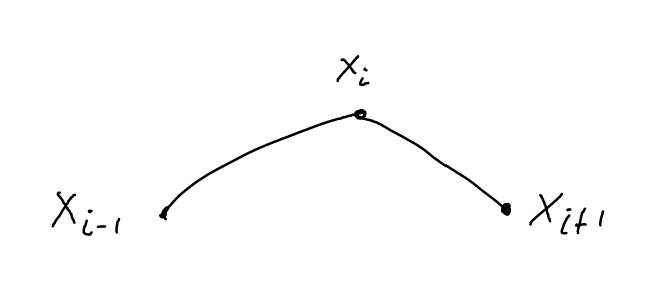
\includegraphics[scale=0.4]{img/base.png}\\
Hay 4 casos posibles:
\begin{enumerate}

\item $x_{i+1} \in \Gamma^+(x_i)$ y $x_i\in \Gamma^+(x_{i-1})$: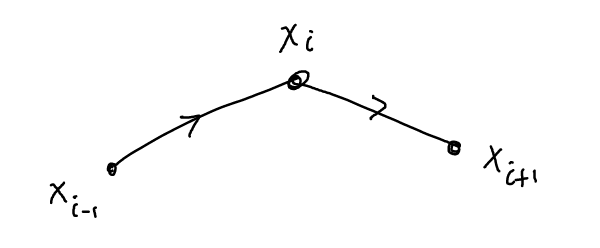
\includegraphics[scale=0.4]{img/forward-forward.png}\\
Como 
\begin{align}
    \left.
    \begin{array}{cc}
    F^*(\overrightarrow{x_i x_{i+1}}) = F(\overrightarrow{x_i x_{i+1}}) + \varepsilon\\
    F^*(\overrightarrow{x_{i-1} x_i}) = F(\overrightarrow{x_{i-1} x_i}) + \varepsilon 
    \end{array}
     \right\} \implies
     \begin{array}{cc}
    out_{F^*}(x_i) = out_F(x_i) + \varepsilon \\
    in_{F*} (x_i) = in_F(x_i) + \varepsilon
    \end{array}
\end{align}
$\therefore out_{F^*} (x_i) - in_{F^*}(x_i) = 0.$\\
Cambiaron los lados que entran y salen de $x_i$.
    
\item $x_{i+1} \in \Gamma^+(x_i)$ y $x_{i-1} \in \Gamma^{-}(x_{i})$: 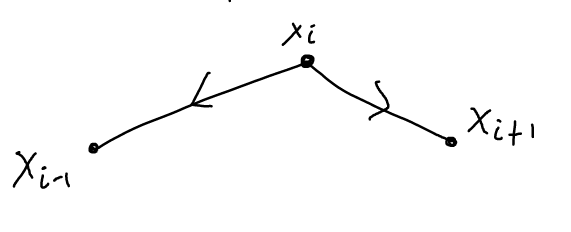
\includegraphics[scale=0.4]{img/backward-forward.png}\\
\begin{align}
    \left.
    \begin{array}{cc}
    F^*(\overrightarrow{x_i x_{i+1}}) = F(\overrightarrow{x_i x_{i+1}}) + \varepsilon\\
    F^*(\overrightarrow{x_{i-1} x_i}) = F(\overrightarrow{x_i x_{i+1}}) - \varepsilon 
    \end{array}
     \right\} \implies
     \begin{array}{cc}
    out_{F^*}(x_i) = out_F(x_i) + \varepsilon -  \varepsilon = out_F(x_i)\\
    in_{F^*} (x_i) = in_F(x_i)
    \end{array}
\end{align}
$\therefore out_{F^*} (x_i) - in_{F^*}(x_i) = 0.$\\
Cambiaron dos lados que salen de $x_i$ y ninguno que entra a $x_i$ cambió.

\item $x_i \in \Gamma^-(x_{i+1})$ y $x_i\in \Gamma^+(x_{i-1}):$ 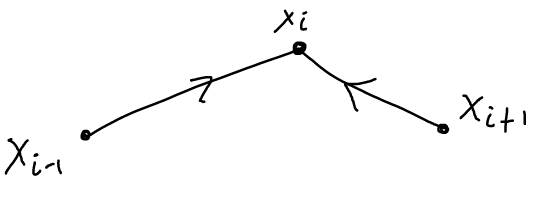
\includegraphics[scale=0.4]{img/forward-backward.png}\\
\begin{align}
    \left.
    \begin{array}{cc}
    F^*(\overrightarrow{x_{i+1} x_i}) = F(\overrightarrow{x_{i+1} x_i}) - \varepsilon\\
    F^*(\overrightarrow{x_{i-1} x_i}) = F(\overrightarrow{x_{i-1} x_i}) + \varepsilon 
    \end{array}
     \right\} \implies
     \begin{array}{cc}
    out_{F^*}(x_i) = out_F(x_i) + \varepsilon -  \varepsilon = out_F(x_i)\\
    in_{F^*} (x_i) = in_F(x_i)
    \end{array}
\end{align}

\item $x_{i}\in \Gamma^-(x_{i+1})$ y $x_{i-1} \in \Gamma^-(x_{i})$: 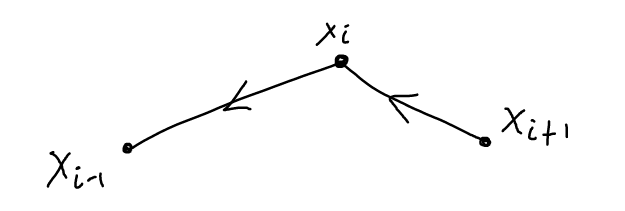
\includegraphics[scale=0.4]{img/backward-backward.png}
\begin{align}
    \left.
    \begin{array}{cc}
    F^*(\overrightarrow{x_i x_{i-1}}) = F(\overrightarrow{x_{i} x_{i-1}}) - \varepsilon\\
    F^*(\overrightarrow{x_{i+1} x_{i}}) = F(\overrightarrow{x_{i+1} x_{i}}) - \varepsilon 
    \end{array}
     \right\} \implies
     \begin{array}{cc}
    out_{F^*}(x_i) = out_F(x_i) + \varepsilon -  \varepsilon = out_F(x_i)\\
    in_{F^*} (x_i) = in_F(x_i)
    \end{array}
\end{align}

\end{enumerate}

Respecto al $v_{F^*}$ tenemos que:\\
Si $x_1 \in \Gamma^+(s)$ entonces
\begin{align}
    V_{F*} &= out_{F^*}(s) - in_{F^*}(s)\\
        &= out_F(s) + \varepsilon - in_{F}(s)\\
        &= v_F + \varepsilon
\end{align}
Si $x_1 \in \Gamma^-(s)$ entonces
\begin{align}
    v_{F^*} &= out_{F^{*}}(s) - in_{F^*}(s)\\
        &= out_F(s) - (in_F(s) - \varepsilon)\\
        &= v_F + \varepsilon
\end{align}
\end{proof}

\begin{lemma}
Sea $N$ un network, $G$ un flujo de $s$ a $t$ y $S$ un corte cualquiera, entonces
\begin{align}
    v_G = G(S, S^c) - G(S^c, S)
\end{align}
\end{lemma}

\begin{proof}
Sea $x\in S$. Vemos que $out_G(x) - in_G(x) = \left\{
    \begin{array}{cc}
     0  &x\neq s\\
     v_G &x = s
    \end{array}
\right.$\\

\begin{align}
    \therefore v_G &= \sum_{x\in S} out(x) - in(x) = \sum_{\substack{x\in S\\xv \in E}} G(x,v) - G(v,x)\\
    &= G(S,V) - G(V,S)  &&\text{Aca usamos: } S \cup S^c = V \wedge S \cap S^c = \varnothing \\
    &= G(S,S) + G(S, S^c) - G(S,S) - G(S^c, S)\\
    &= G(S,S^c) - G(S^c, S)
\end{align}

\end{proof}

\begin{corollary}
El valor del flujo es una cota inferior de la capacidad de un corte $S$ esto es: $v_G \le cap(S)$
\end{corollary}
\begin{proof}
Por restricción de capacidad y conservación, sabemos que \\$G(S, S^c) \le C(S, S^c)$ y $G(S^c, S) \ge 0$ entonces vale:
\begin{align}
v_G &= G(S, S^c) - G(S^c, S)\\
	&\le G(S, S^c)\\
    &\le cap(S)
\end{align}
\end{proof}

\begin{theorem}[\textit{Max-flow min-cut}]
Sea $N = (V,E,C)$ un network, $F$ un flujo de $s$ a $t$ en $N$ y $S$ un corte minimal de $V$ entonces
\begin{align}
    \underbrace{F \text{ es maximal}}_{A} \iff 
    \underbrace{\nexists \text{ caminos } F\text{-aumentantes entre $s$ y $t$}}_{B} \iff
    \underbrace{v_F = mincutcap_S}_{C}
\end{align}
\end{theorem}
\begin{proof}
$C \implies A:$\\
Asumamos $C)$. Sea $S$ un corte con $cap(S) = v_F$\\
Sea $G$ otro flujo. Tenemos por [ref] que
\begin{align} v_G \le cap(S) = v_F \end{align}
de lo que se sigue que $F$ es maximal.\\

Notar que así mismo, $S$ es minimal pues dado un corte cualquiera $T$\begin{align}
    cap(T) \ge v_F = cap(S)
\end{align}
$B \implies C:$\\
Sea $S = \{s\} \cup \{x \in V \mid \exists \text{ camino $F$-aumentante de $s$ a $x$}$\}.
Es claro que $t \notin S$ pues por hipótesis \\$\nexists$ caminos $F$-aumentantes de $s$ a $t$.\\
$\therefore S$ es corte.\\
Como $S$ es corte,
\begin{align}
    v_F = F(S, S^c) - F(S^c, S)
\end{align}
Sea $x \in S$, $y \in S^c$, $\overrightarrow{xy} \in E$. Buscamos $F(xy)$, y vemos que:
\begin{itemize}
    \item $\exists$ un camino F-aumentante $(x_0, x_1,\mathellipsis, x_r)$ entre $s$ y $x$
    \item $\nexists$ un camino $F$-aumentante entre $s$ e $y$
\end{itemize}
Esto es, $(x_0, \mathellipsis, x_r, y)$ no es un camino $F$-aumentante.\\
Como $(x_0, x_1, \mathellipsis, x_r)$ si lo es, y $\overrightarrow{xy} \in E$, concluimos que $\overrightarrow{xy}$ está saturado, ie. \\$F(\overrightarrow{xy}) = C(\overrightarrow{xy})$.
\begin{align}
    \therefore \forall x,y: x \in S \wedge y \in S^c \wedge xy \in E : F(\overrightarrow{xy}) = C(\overrightarrow{xy})\\
    F(S, S^c) = \sum_{\substack{x\in S\\ y \notin S \\\overrightarrow{xy} \in E}} F(\overrightarrow{xy}) = \sum_{\substack{x\in S\\ y \notin S\\ \overrightarrow{xy} \in E}} C(\overrightarrow{xy}) = C(S, S^c) = cap(S)\\
\end{align}
Ahora, veamos el otro caso. Sea $x \in S^c, y \in S, \overrightarrow{xy} \in E$. Buscamos $F(\overrightarrow{xy})$. Con un análisis similar al anterior, teniendo en cuenta que ahora $x\in \Gamma^-(y)$, concluimos $xy$ está vacio ie. $F(\overrightarrow{xy}) = 0$.
\begin{align}
    \therefore \forall x, y : x \in S^c \wedge y \in S \wedge xy \in E : F(\overrightarrow{xy}) = 0\\
    F(S^c, S) = \sum_{\substack{x\not\in S\\ y \in S\\ \overrightarrow{xy} \in E}} F(\overrightarrow{xy}) = \sum_{\substack{x\not\in S\\ y \in S\\ \overrightarrow{xy} \in E}} 0 = 0
\end{align}
Así,
\begin{align}
v_F = F(S, S^c) - F(S^c, S) = cap(S) - 0 = cap(S) = mincutcap_S
\end{align}
Por último, $S$ es claramente minimal.

$A \implies B$:\\
Suponiendo $F$ maximal, supongamos que $B$ es falso, es decir, que existe un camino $F$-aumentante entre $s$ y $t$.\\
Por el lema [\ref{flujo_camino_aumentante}], es posible enviar $\varepsilon$ unidades de flujo por ese camino y obtener un flujo $F^*$ con $v_{F^*} = v_F + \varepsilon$. Esto es absurdo pues $F$ es maximal.
\end{proof}

\begin{algorithm}
\caption{Algoritmo de Edmonds-Karp para hallar flujo maximal}
\begin{algorithmic}
\Require network $N=(V,E,C)$
\Ensure  $(F, v, S)$ donde $F$ es flujo maximal, $v$ es el valor del flujo y $S$ es el corte minimal
\Function{Edmonds-Karp}{$network\ N$}
\State $F = 0, v = 0, \varepsilon(s) = \infty$
\While{$true$} 
    \State $queue\ Q = qEmpty()$
    \State $qEnqueue(Q,s)$
    \State $S := \{s\}$
    \While{$qCnt(Q)$}
        \State $x = qDequeue(Q)$
        \State \ForAll{$z \in \Gamma^{+}(x) \cap S^c$}
        \If{$F(xz) < C(xz)$}
            \State $qEnqueue(Q,z)$
            \State $S = S \cup \{z\}$
            \State $a(z) = x;\ b(z) = 1$
            \State $\varepsilon(z) = min\{\varepsilon(x), C(xz) - F(xz)\}$
        \EndIf
        \EndFor
        \State \ForAll{$z\in \Gamma^{-}(x) \cap S^c$}
        \If{$F(zx) > 0$}
        \State $qEnqueue(Q,z)$
        \State $S = S \cup \{z\}$
        \State $a(z) = x;\ b(z) = -1$
        \State $\varepsilon(z) = min\{\varepsilon(x), F(zx)\}$
        \EndIf
        \EndFor
        \EndWhile
        \State
        \If{$t \in S$}
        \State $q = t;\ \varepsilon = \varepsilon(t);\ v = v+E$
        \While{$q \neq s$}
        \State $p = a(q)$
        \If{$b(q) == 1$}
        \State $F(pq) = F(pq) + \varepsilon$
        \State $F(qp) = F(qp) - \varepsilon$
        \EndIf
        \State q = p;
        \EndWhile
        \Else
        \State \Return{$F, v, S$}
        \EndIf
\EndWhile
\EndFunction
\end{algorithmic}
\end{algorithm}

\begin{theorem}[Teorema de integralidad]\label{integrality}
Sea $N=(V,E,C)$ un network tal que $\forall xy \in E : C(xy) \in \mathbb{Z}$ entonces $\exists$ flujo maximal entero.

En otras palabras, en un network con capacidades enteras encontraremos siempre un flujo maximal entero.
\end{theorem}

\begin{proof}
Lo probaremos por inducción, corriendo el algoritmo de Ford-Fulkerson en $n+1$ pasos, sean $F_0, \mathellipsis, F_n$ los sucesivos flujos obtenidos:\\
Caso base: $F_0 = 0 \in \mathbb{Z}$.\\
Caso inductivo:
$F_k \in \mathbb{Z} \implies F_{k+1} \in \mathbb{Z}$\\
$F_{k+1}$ se construye a partir de $F_k$, cambiando en algunos lados el valor $F_k$ por $F_k \pm \varepsilon$. Por lo tanto, si probamos que $\varepsilon \in \mathbb{Z}$, también tendremos que $F_{k+1} \in \mathbb{Z}$. Luego,
\begin{align}
    \varepsilon = \min\{\epsilon_i\}
\end{align}
y \begin{center}
    $\epsilon_i = \begin{cases} C(\overrightarrow{x_i x_{i+1}}) - F(\overrightarrow{x_i x_{i+1}}) & \text{ si } \overrightarrow{x_i x_{i+1}} \text{ es lado forward}\\
    F(\overrightarrow{x_{i+1} x_i}) & \text{ si } \overrightarrow{x_i x_{i+1}} \text{ es lado backward}
    \end{cases}$
\end{center}
Como las capacidades son todas enteras, $\epsilon_i$ es entero, $\varepsilon$  es entero y por lo tanto $F_{k+1}$.
Esto prueba que si Ford-Fulkerson termina, obtenemos un flujo maximal entero.
Como $v_{F_{k+1}} - v_{F_k} = \varepsilon \in \mathbb{Z} > 0$, por lo tanto $\varepsilon \ge 1$. Esto es, el ``salto" que se produce entre un flujo y el siguiente es discreto.
Como existe una cota superior para el conjunto de valores de flujos posibles (por ej. $cap(S)$), esta sucesión de flujos debe ser finita. 
\end{proof}

\begin{definition}
Dados $a,b\in V$ y un flujo $F$ en un network $N = (V,E,C)$. Definimos a la \emph{distancia (respecto de $\boldsymbol{F}$) de $\boldsymbol{a}$ hasta $\boldsymbol{b}$} como:
\begin{align}
D_F(a,b) = \left\{
    \begin{array}{cc}
         0 & a = b\\
         \#\{x_i x_{i+1} \in E\mid 0\le i < r \}  &\text{si $\{x_0, \mathellipsis, x_r\}$ es el menor camino $F$-aumentante entre $a$ y $b$} \\ 
         \infty &\text{si $\nexists$ camino $F$-aumentante entre $a$ y $b$}
    \end{array}
    \right.
\end{align}
Esto es, el numero de lados del menor camino aumentante relativo a $F$ entre $a$ y $b$.\\
Asimismo, definimos
\begin{itemize}
    \item $d_F(x) \doteq D_F(s,x)$
    \item $b_F(x) \doteq D_F(x,t)$
\end{itemize}
\end{definition}

\begin{lemma}\label{distancias_no_decrecen_EK}
Sea $N=(V,E,C)$ un network y $F_1, F_2, \mathellipsis, F_\ell$ los flujos parciales obtenidos por Edmonds-Karp (supongamos que $F_0 = 0$ es el flujo inicial).\\
Abreviaremos
\begin{align}
    d_k(x) \doteq d_{F_k}(x) \\
    b_k(x) \doteq d_{F_k}(x)
\end{align} entonces tenemos que $\forall x \in V$:
\begin{align}
    d_k(x) \le d_{k+1}(x) \\
    b_k(x) \le b_{k+1}(x)
\end{align}
\end{lemma}

\begin{proof}
$\forall i : 1 \le i \le \ell$ :\\
\begin{enumerate}
    \item
    Sea $A_i \doteq \{x \in V \mid d_i(x) < d_{i-1}(x)\}$, queremos ver que $A_i = \varnothing$ comenzando por notar que $s \notin A_i$ ya que $\forall i: d_i(s) = 0$.\\
    Supongamos que $\exists i : A_i \neq \varnothing$. Sea ese $i$ el mínimo posible. A su vez, sea $x = \min\{d_i(v) \mid v \in A_i \}$, ie. tal que $d_i(x)$ sea mínimo. Entonces, $\forall z : d_i(z) > d_i(x) \implies z\notin A_i$.\\
    Como $d_i(x) < d_{i-1}(x) \le \infty$ tenemos que $d_i(x) < \infty$ y debe haber un camino $F_i$-aumentante de $s$ a $x$. Sea $(x_0, \mathellipsis, x_r)$ el camino mínimo (es decir, con $r = d_i(x)$).\\
    Probemos ahora que $\nexists$ un camino $F_{i-1}$-aumentante de $s$ a $x$, y luego lleguemos a una contradicción.\\
    Sea $z = x_{r-1}$. Como $(x_0,\mathellipsis, x_r)$ es el camino $F_i$-aumentante de menor longitud entre $s$ y $x$ entonces $(x_0, \mathellipsis, x_{r-1})$ es el camino $F_{i}$-aumentante de menor longitud entre $s$ y $z$. Así, como $d_i(z) = r-1$ se sigue que $z \notin A_i$. Concluimos que $d_{i-1}(z) \le d_i(z) < d_i(x) < d_{i-1}(x)$. \\
    $\therefore d_{i-1}(z) \le d_{i-1}(x)-2$.
    Pero consideremos que $d_{i-1}(x) \le d_{i-1}(z) + 1$, ya que se puede ir de $z$ a $x$.
    Como $d_{i-1}(z)+2 \le d_{i-1}(x)$, esto es absurdo.\\
    $\therefore \nexists$ camino $F_{i-1}$-aumentante $(s,\mathellipsis, z, x).$\\
    Ahora la contradicción:\\
    Como existe un camino $(s, \mathellipsis, z, x)$, debe pasar $x \in \Gamma^+(z)$ o bien $x \in \Gamma^-(z)$. La razón por la que no existe un camino $F_{i-1}$ aumentante puede ser alguna de las siguientes:
    \begin{itemize}
        \item $x \in \Gamma^+(z) \wedge F_{i-1}(\overrightarrow{zx}) = C(\overrightarrow{zx})$
        \item $x \in \Gamma^-(z) \wedge F_{i-1}(\overrightarrow{zx}) = 0$ 
    \end{itemize}
    Pero como el camino $F_i$-aumentante si existe,
    \begin{itemize}
        \item $x \in \Gamma^+(z) \wedge F_{i-1}(\overrightarrow{zx}) = C(\overrightarrow{zx}) \wedge F_i(\overrightarrow{zx}) < C(\overrightarrow{zx})$
        \item $x \in \Gamma^-(z) \wedge F_{i-1}(\overrightarrow{zx}) = 0 \wedge F_i(\overrightarrow{zx}) > 0$
    \end{itemize}

    La única forma en que esto puede ocurrir es que al pasar de $F_{i-1}$ a $F_i$ usemos un camino de la forma $(s, \mathellipsis, x, z)$, ya que:
    \begin{itemize}
        \item Si el último lado es backward, $x \in \Gamma^+(z) \wedge F_{i}(\overrightarrow{zx}) < F_{i-1}(\overrightarrow{zx})$ (primer razón).
        \item Si el último lado es forward, $x \in \Gamma^-(z) \wedge F_{i}(\overrightarrow{xz}) > F_{i-1}(\overrightarrow{xz})$ (segunda razón).
    \end{itemize}
    Como usamos Edmonds-Karp, este camino tiene longitud mínima.
    Entonces $d_{i-1}(z) = d_{i-1}(x) + 1$. Pero sabemos que $d_{i-1}(x) + 1  = d_{i-1}(z) \le d_{i-1}(x) - 2$. Esto es una contradicción. Concluimos:
    \begin{align}
        \nexists i : A_i \neq \varnothing
        \equiv
        \forall i : A_i = \varnothing
    \end{align}
    Es decir, $\forall i, x : x \in V : d_{i-1}(x) \le d_i(x)$
    \item
    Similarmente, podemos construir un $B_i = \{x \in V \mid b_i(x) < b_{i-1}(x) \wedge i \ge 1\}$ y probar que
    \begin{align}
    \forall i : B_i = \varnothing && \text{ie.}\\
    \forall i, x : x \in V : b_{i-1}(x) \le b_i(x)
    \end{align}
    \end{enumerate}
\end{proof}

\begin{theorem}[Complejidad del algoritmo de Edmonds-Karp] 
El algoritmo de Edmonds-Karp para encontrar un flujo maximal y un corte minimal en un network es de complejidad $\mathcal{O}(n m^2)$
\end{theorem}
\begin{proof}
Notemos que al construir cada $F_i$ pasa una de las siguientes:
\begin{itemize}
    \item Al menos un lado forward se satura.
    \item Al menos un lado backward se vacía.
\end{itemize}
Llamamos \emph{crítico} a un tal lado.
Supongamos que un lado con vértices $x$ y $z$ se volvió crítico en el paso $i$. Antes de que pueda volverse crítico deberá usarse para el otro lado (si se usó como forward, debe usarse como backward, y viceversa). Supongamos que sucede eso en el paso $j > i$.\\
Así, $(s, \mathellipsis, z, x)$ es un camino mínimo en el paso $i$, y $(s,\mathellipsis, x, z)$ en el paso $j$.
Como el camino $F$-aumentante de $s$ a $t$ en el paso $j$ contiene a $z$:
\begin{align}
    d_j(t) = d_j(z)+b_j(z)
    \end{align}
Además, $z$ está después de $x$ en este camino:
\begin{align}
    d_j(t) = d_j(x) + 1 + b_j(z)
\end{align}
Por el lema [\ref{distancias_no_decrecen_EK}], sabemos que $d_{i-1}(x) \le d_i(x)$ (haciendo la sustitución: $i-1 := i \wedge i := j$) y:\begin{align}
    d_j(t) \ge d_i(x) + 1 + b_i(z)
\end{align}
Y ahora, en el paso $i$, $z$ está antes que $x$:
\begin{align}
    d_j(t) \ge d_i(x) + 1 + 1 + b_i(x)
\end{align}
Y entonces:
\begin{align}
    d_j(t) \ge d_i(t) + 2
\end{align}
Concluimos que si un lado se vuelve crítico, antes de que pueda volver a hacerlo, la distancia entre $s$ y $t$ debe aumentar en al menos $2$.\\
Por lo tanto, un lado puede volverse crítico a lo sumo $\frac{n+1}{2} \in \mathcal{O}(n)$ veces.
Sabemos que en la construcción de cada $F_i$ al menos un lado se vuelve crítico. Así, tenemos que \begin{align}
    \# F_i &\le m * \# \text{veces que puede volverse crítico}\\
    \# F_i &\in \mathcal{O}(nm)
\end{align}
Cada corrida consiste en construir un $F_i$ mediante $BFS \in \mathcal{O}(m)$.\\
 $\therefore$ La complejidad del algoritmo Edmonds-Karp es $\mathcal{O}(m) * \mathcal{O}(nm) = \mathcal{O}(nm^2)$
\end{proof}

\subsection{Dinic-Even}

\begin{algorithm}
\caption{Algoritmo de Dinic-Even para encontrar flujo maximal}
\begin{algorithmic}
\Require network $N=(V,E,C)$
\Ensure  $F$ un flujo maximal
\Function{Dinic}{$network\ N$}
\State $F = 0$
\State $L$ = \Call{LayeredNetwork}{$N, F$} \Comment{ Construir un network auxiliar por niveles $L$ basado en $F$ y $N$}
\While{$t \notin L$}
    \State $F$ += \Call{BlockingFlow}{$L$}
    \State $L$ = \Call{LayeredNetwork}{$N, F$}
\EndWhile
\State \Return{$F$}
\EndFunction

\State

\Function{BlockingFlow}{layered network $L$}
\State $len = d_L(s,t)$
\State vertex path $P = [s]$
\State $G = 0$ \Comment{Este será flujo bloqueante}
    \While{$true$}
    \State $i = 0$
        \While{$i < len$}
            \State $v = P[i]$
            \If{$\Gamma^+(v) \neq \varnothing$}
                \Comment{Avanzar}
                \State $P$ += algún vecino de $v$
                \State $i$ += $1$
            \ElsIf{$v \neq s$}
                \Comment{No podemos llegar a $t$: Retroceder}
                \State $E_L$ -= $\overrightarrow{P[i-1] P[i]}$
                \State $i$ -= $1$
            \Else
                \State \Return{$G$} \Comment{Solo terminamos cuando $\Gamma^+(s) = \varnothing$}
            \EndIf
        \EndWhile
    
        \Comment{Llegamos a $t$: Incrementar}
        \State $\varepsilon = \min_{0\le i < len} \{ C(\overrightarrow{P[i] P[i+1]}) - G(\overrightarrow{P[i] P[i+1]})\}$
        \For {$i \in \{0, \mathellipsis, len-1\}$}
            \State $G(\overrightarrow{P[i] P[i+1]})$ += $\varepsilon$
            \If {$C(\overrightarrow{P[i] P[i+1]}) = G(\overrightarrow{P[i] P[i+1]})$}
                \State $E_L$ -= $\overrightarrow{P[i] P[i+1]}$
            \EndIf
        \EndFor
    \EndWhile
\EndFunction
\end{algorithmic}
\end{algorithm}

\begin{definition}[Network por niveles]
Un network $N = (V,E,C)$ es un \emph{network por niveles} si:
\begin{align}
 V &= \bigcup_{i=0}^r V_i \\
 E &= \{\overrightarrow{xy} \mid \forall i: 0 \le i \le r : x \in V_i \wedge y \in V_{i+1}\}
 \end{align}
 tal que $\forall i, j : 0 \le i < j \le r \wedge i \neq j : V_i \cap V_j = \varnothing$ \\
Y con $V_0 = \{s\} \text{ y } V_r = \{t\}$

Es decir, solo hay lados entre vértices de distintos niveles siendo el primer nivel el de $s$ y el último el de $t$.
\end{definition}

\begin{definition}[Network residual]
Dado un network $N = (V_N, E_N, C_N)$ y un flujo $F_N$, el \emph{network residual} $R$ = $R_F$ = $R_{F_N} = (V_R, E_R, C_R)$ es el network tal que:
\begin{itemize}
    \item $V_R = V_N$
    \item $(\overrightarrow{xz}) \in E_R \iff 
    \left\{ 
    \begin{array}{cc}
    \overrightarrow{xz} \in E_N \wedge F_N(\overrightarrow{xz}) < C_N(\overrightarrow{xz})     & \text{caso \textit{forward}} \\
    \text{o bien}  & \\
    \overrightarrow{zx} \in E_N \wedge F_N(\overrightarrow{zx}) > 0 & \text{caso \textit{backward}}
    \end{array}
    \right.$
    \item $C_R(\overrightarrow{xz}) = \left\{
    \begin{array}{cc}
        C_N(\overrightarrow{xz}) -
        F_N(\overrightarrow{xz})   & \text{caso \textit{forward}}\\
        F_N(\overrightarrow{zx})   & \text{caso \textit{backward}}
    \end{array}
    \right.
    $
\end{itemize}
\end{definition}

\begin{definition}[Network auxiliar por niveles o \textit{level graph}]
Dado un network residual $R = R_F = R_{F_N} = (V_R, E_R, C_R)$ definimos al \emph{network auxiliar por niveles} o $\boldsymbol{level}$  $\boldsymbol{graph}\ L = L_F = (V_L, E_L, C_L)$ de la siguiente forma:
\begin{itemize}
    \item $V_L = \{ x\in V_R \mid d_F(x) < d_F(t)\} \cup \{t\}$
    \item $E_L = \{\overrightarrow{xy} \in E_R \mid d_F(x) + 1 = d_F(y)$\}
    \item $C_L = C_R$
\end{itemize}

\end{definition}

\begin{definition}[Flujo bloqueante]
Un \emph{flujo bloqueante} o $\boldsymbol{blocking}$  $\boldsymbol{flow}$ es un flujo tal que todos los caminos dirigidos de $s$ a $t$ tienen al menos un lado saturado.
\end{definition}

\begin{algorithm}
\caption{Pseudocódigo de Algoritmos tipo Dinic}
\begin{algorithmic}
\State $F = 0$
\While{$d_F(t) < \infty$}
    \State Construir un \textit{level graph} $L = L_F$
    \State Hallar flujo bloqueante $G$ en $L$
    \State Modificar $F$ en $N$ de acuerdo a $G$
\EndWhile

\end{algorithmic}
\end{algorithm}

\begin{theorem}
Entre dos level graphs consecutivos la distancia entre $s$ y $t$ aumenta.
\end{theorem}

\begin{proof}
Sean $A$ y $B$ dos networks auxiliares consecutivos. Probaremos que $d_A(t) < d_B(t)$. 
Sabemos que $d_A(t) \le d_B(t)$ por el lema [\ref{distancias_no_decrecen_EK}] de Edmonds-Karp (seguimos utilizando el camino más corto).
Debemos entonces probar que $d_A(t) \neq d_B(t)$.\\
Primero, observemos que $s, x_1, \mathellipsis, x_{r-1}, t$ es un camino dirigido no saturado en $A \iff$ no lo es en $B$, puesto que si es no saturado en $A$ el flujo bloqueante satura uno de sus lados, y si no lo es en $B$ entonces no estaba en $A$ (el flujo bloqueante lo hubiera saturado).\\
Sea $s, x_1, \mathellipsis, x_{r-1}, t$ el mínimo camino dirigido no saturado en $B$. Como dijimos, este camino no estaba en $A$. Esto puede darse por dos razones:

\begin{enumerate}
    \item Caso 1: $\exists i : x_i \in V_B : x_i \notin V_A$: Falta un vértice $x_i$ en $A$ que si está en el $B$ (notar que $x_i \neq s,t$).\\
    Entonces $d_A(t) \le d_A(x_i)$, ya que si la distancia fuese menor hubiera estado en $A$. Por el lema de E-K [\ref{distancias_no_decrecen_EK}], $d_A(x_i) \le d_B(x_i)$.\\
    Así, $d_{A}(t) \le d_{A}(x_i) \le d_{B}(x_i) < d_{B}(t)$ ($x_i$ está antes de $t$ en el camino en $B$). Así, $d_A(t) < d_B(t)$.
    
    \item Caso 2: $\exists i : \overrightarrow{x_{i-1} x_i} \notin E_A$: falta un lado $\overrightarrow{x_{i-1} x_{i}}$ pero ningún vértice. 
    Esto puede pasar por dos razones (correspondientes a la definición de $E_R$ y $E_A$). \\
    Tomemos el mínimo $i$ tal que $\overrightarrow{x_{i-1} x_{i}} \notin E_A$:
    
    \begin{enumerate}
    \item Caso A: El lado está saturado o vacío (en $N$).\\
    Como en $E_B$ este lado si está, al incrementar el flujo en $A$ debimos usarlo en el otro sentido: con un camino $s, \mathellipsis, x_i, x_{i-1}, \mathellipsis, t$. Así,
    \begin{align}
        d_B(t)
        &= d_B(x_i) + b_B(x_i)\\
        &= d_B(x_{i-1}) + 1 + b_B(x_i)\\
        &\ge d_A(x_{i-1}) + 1 + b_A(x_i)\\
        &\ge d_A(x_{i-1}) + 1 + b_A(x_{i-1}) + 1\\
        &\ge d_A(t) + 2\\
        &> d_A(t)
    \end{align}
    Como en E-K.
    %$\left.
    %\begin{array}{cc}
    %(\overrightarrow{x_{i-1} x_{i}}) \notin  E_{R_{A}}     &  \\
    %(\overrightarrow{x_{i-1} x_{i}}) \in E_{R^*_{B}}     & 
    %\end{array}
    %\right\}$
    %solo puede ocurrir si $(\overrightarrow{x_{i} x_{i-1}}) \in E_L$\\
    %Veamos lo anterior:\\
    %Supongamos que 
    %$(\overrightarrow{x_{i+1} x_i}) \in E_L$, luego $d_A(x_{i+1}) + 1 = d_A(x_i)$\\
    %Entonces, $d_A(t) = d_A(x_i) + b_A(x_i)$. Pero $\overrightarrow{(x_i x_{i+1}})$ es el primer %lado que no está en $E_L$
    %\begin{align}
    %\forall k : 0 \le k < i &: (\overrightarrow{x_{k-1} x_{k}}) \in E_L \implies \\
    %\forall j : j < i &: d_A(x_j) = j 
    %\end{align}
    %Entonces, $(\overrightarrow{x_{i-1} x_{i}}) \notin E_{R_A} \wedge (\overrightarrow{x_{i-1} x_{i}}) \in E_{R^{*}_B}$
         
    \item Caso B: El lado no está saturado ni vacío: $d_A(x_i) + 1 \neq d_A(x_{i-1})$\\
    Esto significa que $d_A(x_{i}) \le d_A(x_{i-1}) + 1$ (si no, como el lado no esta saturado ni vacío, estaría en $E_A$).
    $\therefore d_A(x_i) < d_A(x_{i-1}) + 1$. Como el camino es mínimo en $B$,
    \begin{align}
        d_B(t)
        &= d_B(x_i) + b_B(x_i)\\
        &= d_B(x_{i-1}) + 1 + b_B(x_i)\\
        &\ge d_A(x_{i-1}) + 1 + b_A(x_i)\\
        &\ge d_A(x_i) + 1 + b_A(x_i)\\
        &\ge d_A(t) + 1\\
        &> d_A(t)
    \end{align}
    %Pero $d_A(x_{i-1}) = i-1$ (pues $\forall j < i : d_A(x_j) = j$\\
    %Por lo tanto, $d_A(x_{i}) \neq  i-1 +1 = i$, pero como $d_A(x_{i}) \le d_B(x_{i}) = i$, 
    %tenemos que $d_A(x_{i}) < i$\\
    %$\therefore d_A(t) = d_A(x_{i}) + b_A(x_{i}) < i + b_A(x_{i}) \le i + b_B(x_{i}) = d_B(x_{i}) + b_B(x_{i}) = d_B(t)$\\
    %$\therefore d_A(t) < d_B(t)$
    \end{enumerate}
    %Volviendo al caso $A$, tenemos que $d_A(x_i) + 1 = d_A(x_{i-1}) = i-1$\\
    %$\therefore d_A(x_i) = i - 2 < i$ y vale la prueba de 2B.
\end{enumerate}
\end{proof}

\begin{theorem}
La complejidad del paso de flujo bloqueante en el algoritmo de Dinic-Even es $\mathcal{O}(nm)$
\end{theorem}
\begin{proof}
Sean \begin{itemize}
    \item A := 'Avanzar'
    \item R := 'Retroceder'
    \item I := 'Incrementar $G$'
\end{itemize}
Una corrida se corresponde a:
$A^*(A^*R^*)^*I$.\\
Consideremos entonces las palabras de la forma $A^*x$ (con $x \in \{ R, I \}$).
Necesitamos saber cuántas palabras hay y cuál es la complejidad de cada una.
Tengamos en cuenta lo siguente:
\begin{itemize}
    \item $compl$(A) = $\mathcal{O}(1)$
    \item $compl$(R) = $\mathcal{O}(1)$
    \item $compl$(I) = $\mathcal{O}(n)$. 
\end{itemize}

Teniendo en cuenta que R borra un lado del \textit{level graph} y que I también borra al menos un lado (pues al incrementar el flujo se satura al menos un lado) tenemos que:
\begin{align}
    \#palabras(A^*x) \le m
\end{align}

Veamos ahora la complejidad de cada palabra:
\begin{align}
\underbrace{A\mathellipsis A}_j R &\rightarrow \underbrace{\mathcal{O}(1)+\mathellipsis+\mathcal{O}(1)}_j+ \mathcal{O}(1) = \mathcal{O}(j)\\
\underbrace{A\mathellipsis A}_j I &\rightarrow \mathcal{O}(j) + \mathcal{O}(n)
\end{align}
Estamos en un \textit{level graph} y A mueve el pivot $p$ desde $p$ hasta un vecino de $p$. Por lo tanto, A incrementa en 1 el nivel de $p$. Luego de a lo sumo $n$ Avanzar debo llegar a $t$ (o se produce un I o bien hay que Retroceder). Luego $j \le n$

\begin{align}
    \therefore compl(\text{A...AR}) &= \mathcal{O}(j) = \mathcal{O}(n)\\
    compl(\text{A...AI}) &= \mathcal{O}(j) + \mathcal{O}(n)\\
    &= \mathcal{O}(n) + \mathcal{O}(n)\\
    &= \mathcal{O}(n)
\end{align}

Conclusión: $\# palabras \in \mathcal{O}(m)\ \wedge \  compl(palabra) \in \mathcal{O}(n) \implies$
Complejidad del paso de flujo bloqueante del algoritmo de Dinic-Even es $\mathcal{O}(nm)$

\end{proof}

\begin{theorem}
La complejidad del algoritmo de Dinic-Even es $\mathcal{O}(n^2 m)$
\end{theorem}
\begin{proof}
En [ref] vimos que la distancia de $s$ a $t$ en level graphs consecutivos aumenta.\\
$\therefore$ Hay a lo sumo $n-1$ \textit{level graphs}.\\
Tambien vimos que la complejidad del paso bloqueante es $\mathcal{O}(nm)$.
\end{proof}

\begin{definition}
Un network $N = (V,E,C)$ se dice unitario si tiene capacidad $1$ en todos sus lados.\\
$\forall \overrightarrow{xy} \in E : C(\overrightarrow{xy}) = 1$ \\
$\forall x \neq s,t : |\Gamma^+(x)| = 1 \veebar |\Gamma^-(x)| = 1$
\end{definition}
\begin{theorem}
Dinic en un network unitario tiene complejidad $\mathcal{O}(m\sqrt{n})$
\end{theorem}

\begin{proof}
Supongamos que hago $\sqrt{n}$ flujos bloqueantes y el algoritmo aún no termina.
Sea $F$ el flujo que tenemos. Notemos que $F \in \mathbb{Z}$ y que $R_F$ es unitario:
\begin{itemize}
    \item Si $F < C$, $C' = 1$
    \item Si no, $C' = F = 1$
\end{itemize}
Sea $G$ el flujo maximal en $R_F$ obtenido por Dinic.
Como es flujo, $\forall x \neq s,t : out_G(x) = in_G(x)$
Como $C' \le 1$:
\begin{itemize}
    \item si $|\Gamma^-(x)| = 1, in_G(x) \le 1$, es decir $in_G(x) = 0$
\end{itemize}
\end{proof}

\subsection{Wave}
En Edmonds-Karp y Dinic el invariante es que $F$ es flujo, el algoritmo transforma un flujo en otro, y se detiene cuando no hay mas caminos aumentantes (E-K) o no hay mas caminos bloqueantes (Dinic).
Varios algoritmos invierten el esquema: se parte de un pseudo-flujo bloqueante, se lo va transformando en otros pseudo-flujos bloqueantes, hasta obtener un flujo propiamente dicho.

Wave: como $MKM$ pero desde $s$.
Veamos el paso bloqueante:
Sea $(x_0 = s, x_1, \mathellipsis, x_r = t)$ es el orden $BFS$ de la construcción de este network auxiliar.
\begin{algorithm}
\begin{algorithmic}
\Function{Paso bloqueante de Wave}{network N}
\State $G  = 0$
\For{$x\in V$}
\State $D(x) = 0$ \Comment{desbalance in-out}
\EndFor
\For{$x \neq s \wedge x\in V$}
\State $D(x) = 0$
\EndFor
\For{$x \neq s \wedge x \in V$} 
\State $B(x) = false$ \Comment{vértice bloqueado}
\State $A(x) = \varnothing$ \Comment{vértices que le mandan}
\EndFor
\For{$x \in \Gamma^+(s)$}
\State $G(\overrightarrow{sx}) = C(\overrightarrow{sx})$
\State $D(x)$ += $C(\overrightarrow{sx})$
\State $D(s)$ -= $C(\overrightarrow{sx})$
\State $A(x) = \{s\}$
\EndFor
\While{$D(s) + D(t) \neq 0)$}
\For{$x \in [x_1,\mathellipsis,x_{r-1}]$} \Comment{forward wave}
\If{$D(x) > 0$}
\State{$\Call{forwardBalance}{x}$}
\EndIf
\EndFor
\For{$x \in [x_{r-1} \mathellipsis, x_1]$} \Comment{backward wave}
\If{$D(x) < 0 \wedge B(x)$}
\State{$\Call{backwardBalance}{x}$}
\EndIf
\EndFor
\EndWhile
\EndFunction
\end{algorithmic}
\end{algorithm}

\begin{algorithm}
\begin{algorithmic}
\Function{forwardBalance}{vertex x}
\While{$D(x) > 0 \wedge \Gamma^+(x) \neq \varnothing$}
\State elegimos $z \in \Gamma^+(x)$
\If{B(z)}
\State{$\Gamma^+(x) := \Gamma^+(x) - \{z\}$}
\Else
\State $m = min\{D(x), C(\overrightarrow{xz}) - G(\overrightarrow{xz})\}$
\State $G(\overrightarrow{xz}$ += $m$
\State $D(x)$ -= $m$
\State $D(z)$ += $m$
\State $A(z) = A(z) \cup \{x\}$
\If{$G(\overrightarrow{xz}) == C(\overrightarrow{xz})$}
\State $\Gamma^+(x) := \Gamma^+(x) - \{z\}$
\EndIf
\If{$D(x) > 0$}
\State $B(x) := true$
\EndIf
\EndIf
\EndWhile
\EndFunction
\end{algorithmic}
\end{algorithm}

\begin{algorithm}
\begin{algorithmic}
\Function{backwardBalance}{vertex x}
\While{$D(x) > 0$}
\State elegimos $z \in A(x)$
\State $m = min\{D(x), G(\overrightarrow{zx})\}$
\State $G(\overrightarrow{zx}$ -= $m$
\State $D(x)$ -= $m$
\State $D(z)$ -= $m$
\If{$G(\overrightarrow{zx}) == 0$}
\State $A(x) := A(x) - \{z\}$
\EndIf
\EndWhile
\EndFunction
\end{algorithmic}
\end{algorithm}

\begin{theorem}
La complejidad del algoritmo de Wave es $\mathcal{O}(n^3)$
\end{theorem}

\begin{proof}
Wave es de tipo Dinic. Tiene $\mathcal{O}(n)$ networks auxiliares. Probemos que el paso bloqueante es $\mathcal{O}(n^2)$
Al correr el paso bloqueante hacemos una serie de \Call{forwardBalance}{x} y \Call{backwardBalance}{x}.
Al hacer \Call{ForwardBalance}{x} procesamos lados $\overrightarrow{xz}$ de dos categorias posibles:
\begin{itemize}
    \item Categoría T(otal): al procesarlo, $G(\overrightarrow{xz}) = C(\overrightarrow{xz})$. Es decir, se satura o vacía el lado.
    \item Categoría P(arcial): al procesarlo, $G(\overrightarrow{xz}) < C(\overrightarrow{xz})$
\end{itemize}
En los T se remueve de $\Gamma^+(x)$. Solo se entra una vez a T.
El total de lados de categoria T sobre todos los \Call{forwardBalance} sobre todos las olas es $\mathcal{O}(m)$.
De los de categoría P hay a lo sumo uno en cada \Call{forwardBalance}{x}:

$\#$ lados en cat P $\le \#FB$ totales.\\
En una ola hacia adelante hay a lo sumo $(n-2)$ FB(x).
En una de estas olas, puede pasar:
\begin{itemize}
    \item Todos los vértices quedan balanceados.
    \item Queda alguno no balanceado.
\end{itemize}
Toda ola bloquea al menos un vértice.
Como los vértices nunca se desbloquean, hay $\mathcal{O}(n)$ olas hacia adelante.\\
Entonces:
\begin{align}
\#FB &\le (n-2) \# olas
     \le (n-2) \mathcal{O}(n) = \mathcal{O}(n^2)
\end{align}

\text{Complejidad de todos las olas hacia adelante} = \# lados tipo T + \# lados tipo P\\
= $\mathcal{O}(m) + \mathcal{O}(n^2) = \mathcal{O}(n^2)$

Olas hacia atrás:
En los BB(x) también hay dos categorias:\begin{itemize}
    \item T: $G(\overrightarrow{zx})  = 0$
    \item P: $G(\overrightarrow{zx}) > 0$
\end{itemize}
Hay a lo sumo uno de tipo $P$ en cada BB(x).\\
$\#$ tipo P $\le \#$ BB(x)
$\le \mathcal{O}(n) \cdot \#$ olas hacia atras \\
$\le \mathcal{O}(n) \cdot \#$ olas hacia adelante
$\le \mathcal{O}(n) \cdot \mathcal{O}(n)$\\

Tipo T:
Si $\overrightarrow{zx}$ es de tipo T, $z$ se remueve de $A(x)$
¿Cuántas veces puedo agregar a $z$ a $A(x)$ luego de esto?
Necesito que $z$ le mande flujo a $x$ para que pase.
Pero solo hacemos BB(x) si $x$ está bloqueado y si $x$ está bloqueado, como nunca se desbloquea, $z$ no le puede mandar flujo.\\
Así, hay a lo sumo $m$ lados de tipo T y $\#$ olas hacia atrás $\le \#$ tipo T $+ \#$ tipo P
$\le \mathcal{O}(m) + \mathcal{O}(n^2)
\le \mathcal{O}(n^2)$
\end{proof}

\begin{lstlisting}[language=Python]
# levels = [lvl_1, ...., lvl_r]
# where lvl_k contains vertices in the k-th level
# and lvl_0 = [s], lvl_r = [t]
def blockingFlow(AN):
    vs = concat(levels)
    D(s) = CAP({s})
    FB(s)
    while D(s) + D(t) is not 0:
        for v in vs if not B(v):
            FB(v)
        for v in reverse(vs) if B(v):
            BB(v)

def FB(v):
    for w in FNeighbours(v) if D(v) > 0:
        if B(w) or g(v,w) is c(v,w):
            continue
        m = min(D(v), c(v,w)-g(v,w))
        g(v,w) += m
        D(v) -= m
        D(w) += m
    if D(v) > 0:
        B(v) = true
        
def BB(v):
    for w in BNeighbours(v) if D(v) > 0:
        if g(w,v) is 0:
            continue
        m = min(D(v), g(w,v))
        g(w,v) -= m
        D(v) -= m
        D(w) += m
\end{lstlisting}
